\documentclass[12pt]{article}
\usepackage{fancyhdr,epsfig,graphics,tabularx,times}
\pagestyle{empty}
\topmargin=-0.75in
\oddsidemargin=-0.5in
\textwidth=7.5in
\textheight=10.25in
\parindent=0.0in
\parskip=10pt
\linespread{1.0}

\renewcommand{\labelenumi}{(\alph{enumi})}
\renewcommand{\thefigure}{\arabic{section}.\arabic{figure}}
\def\thesection{Problem \#\arabic{section}}

\begin{document}
{\bf BME154L - Exam \#1}\hfill Name:\underline{\hspace*{3.0in}}



\vspace*{0.5in}

\centerline{\LARGE BME154L (Palmeri)}
\vspace*{0.25in}
\centerline{\LARGE Spring 2012}
\vspace*{0.25in}
\centerline{\LARGE Exam \#1}
\vspace*{0.25in}

{\bf Instructions:} 
\begin{itemize}
\item Write your name at the top of each page.
\item Show all work (this is {\it critical} for partial credit!).
\item \underline{Remember to include units with all answers and label all plot axes.}
\item Clearly box all answers.
\item Assume that all components are ideal unless otherwise stated.
\item Assume that op amps rail at $\pm$ 12 V unless otherwise stated.
\end{itemize}

\begin{center}
\begin{tabular}{cc}
\includegraphics[width=0.39\linewidth]{avery.jpg} &
\includegraphics[width=0.3\linewidth]{ziva.jpg} \\
\end{tabular}

Avery \& Ziva wish you good luck!!
\end{center}


\emph{In keeping with the Duke Community Standard, I have neither given nor received aid in completion of this examination.}

\vspace*{0.5in}

Signature:\underline{\hspace*{3.0in}}


\clearpage

{\bf BME154L - Exam \#1}\hfill Name:\underline{\hspace*{3.0in}}



\section{15 points}

\begin{center}
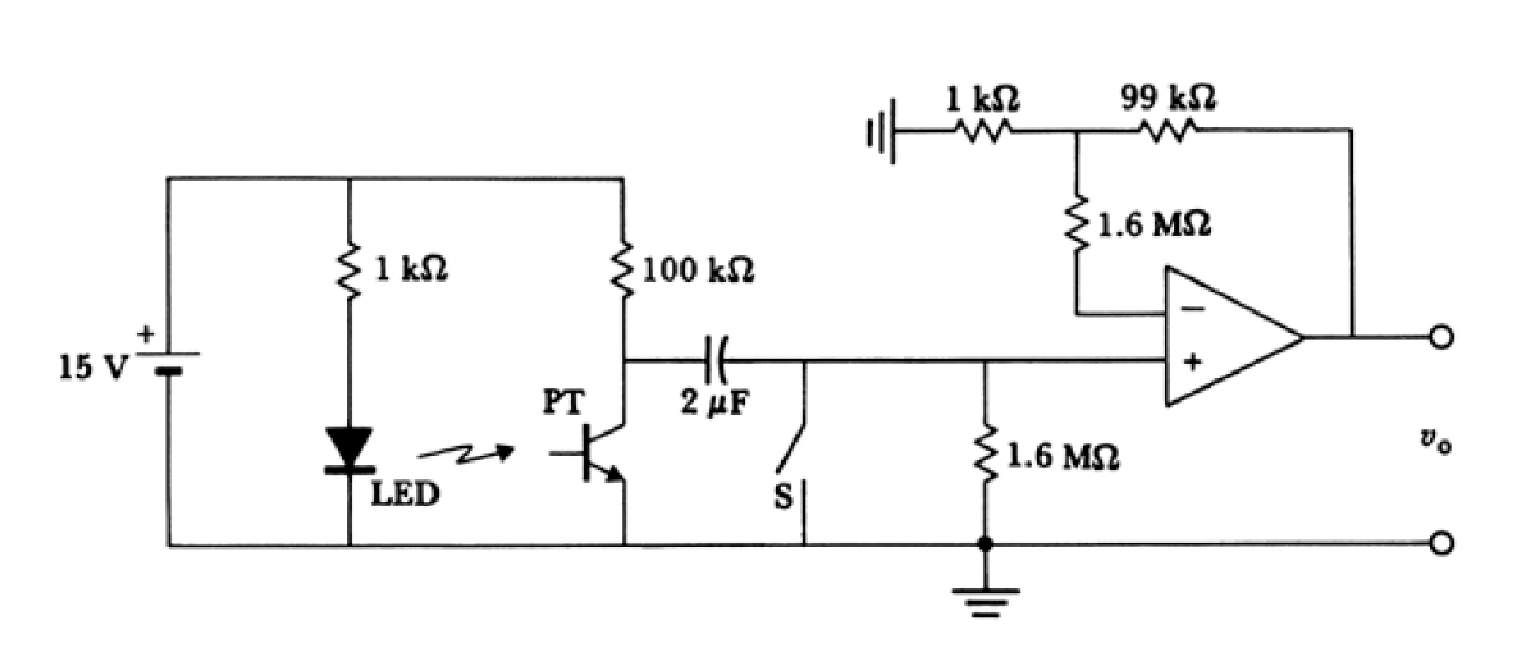
\includegraphics[width=0.5\linewidth]{photo_detect_ckt.eps}
\end{center}

Above is a photodetection circuit for a photoplethysmograph...
\begin{enumerate}
    \item \emph{Briefly} describe:
        \begin{enumerate}
        \item[1.] The purpose of a photoplethysmograph, 
        \item[2.] The physical principles underlying its function, including the relationship between the power emitted from the LED and the power detected by the phototransistor (PT).
        \end{enumerate}
    \item What is the purpose of the 2 $\mu$F capacitor in the circuit?
    \item What is the purpose of the op amp in the circuit?
\end{enumerate}

\clearpage

{\bf BME154L - Exam \#1}\hfill Name:\underline{\hspace*{3.0in}}



\clearpage

{\bf BME154L - Exam \#1}\hfill Name:\underline{\hspace*{3.0in}}



\section{15 points}

\begin{enumerate}
\item Sketch the frequency power spectrum for a delta function.
\item Sketch the frequency power spectrum for white noise.
\item How can two signals that are very different in the time domain have the
same power spectra?
\item The sliding window averager can be implemented as a convolution operation
between your signal and a RECT function, where the width of the RECT is a
function of the number of samples in your averaging window.  Based on this
knowledge, a sliding window averager behaves like what type of filter?  Justify
your answer using the convolution property in the frequency domain (sketches
are fine/preferred over lots of words!).
\end{enumerate}

\clearpage

{\bf BME154L - Exam \#1}\hfill Name:\underline{\hspace*{3.0in}}



\clearpage

{\bf BME154L - Exam \#1}\hfill Name:\underline{\hspace*{3.0in}}



\section{10 points}

%\item Why is digital data transmission more robust than analog data transmission?
%\item Why are checksums used when transmitting/receiving data?
A data transmission line has a throughput of 1 Mbit/s.  A doctor wants to
remotely monitor respiratory rate using tidal volumes ($\approx$ 500 mL) from
an intubation tube using a pneumotachometer.  The default temporal sampling
rate on the pneumotachometer is 100 kHz, but with 32-bit precision per sample,
the bandwidth of the transmission line will be exceeded.  
\begin{enumerate}
    \item What does a pneumotachometer directly measure, and how is that useful in the content of measuring tidal volumes?
    \item What can be done to reduce the amount of data that is
transmitted without compromising the ability to accurately report respiratory
rate. 
\end{enumerate}

\clearpage

{\bf BME154L - Exam \#1}\hfill Name:\underline{\hspace*{3.0in}}



\clearpage

{\bf BME154L - Exam \#1}\hfill Name:\underline{\hspace*{3.0in}}



\section{10 points}

A clinician is using thermodilution methods to measure the cardiac output for a
patient; unfortunately the clinician is a bit sloppy and has an error of
$\pm$10\% on the estimated bolus volume injected and a $\pm$ 20\% error on the
initial temperature of the bolus after rapid injection.  What are the maximum
errors associated with the calculated flow rates associated with these two
measurement errors?

\clearpage

{\bf BME154L - Exam \#1}\hfill Name:\underline{\hspace*{3.0in}}



\section{15 points}

\begin{center}
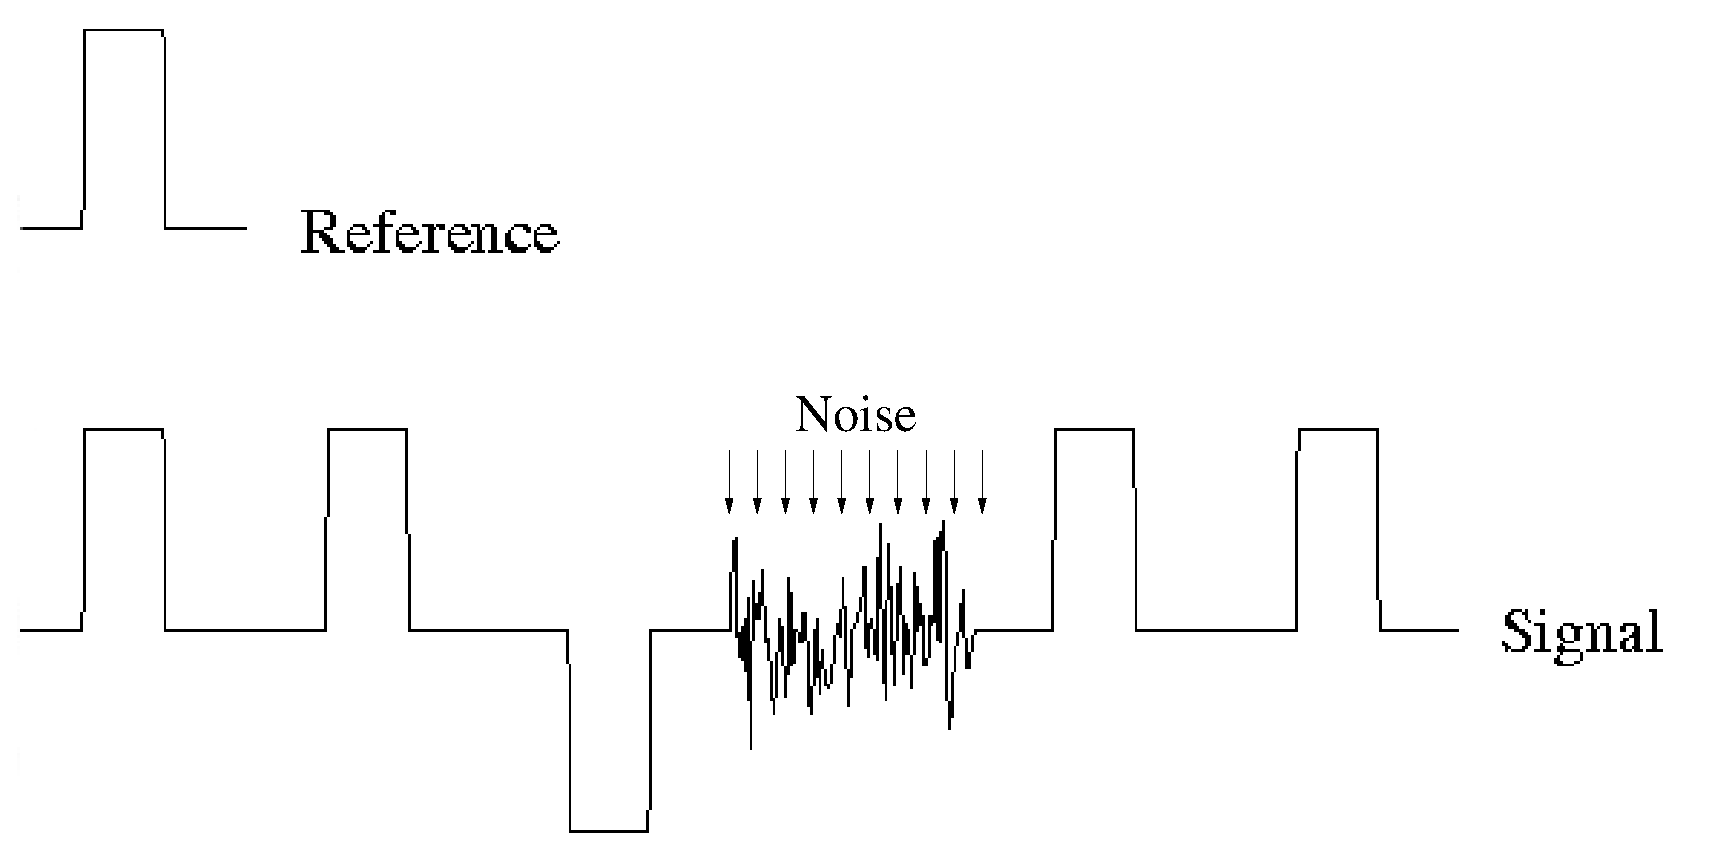
\includegraphics[width=0.5\linewidth]{corrfig.eps}
\end{center}

\begin{enumerate}
\item Sketch the cross correlation function between the signal above and the
specified reference.
\item Assuming that the ``true'' signal includes the periodic RECT waveforms,
sketch the block diagram for a device that will remove regions of noise like
that shown in the middle of the signal without distorting the RECT waveforms;
you can either use the signal, your correlation signal, or both signals as the
input to your device.  \emph{The logic and progression of your signal
processing steps is more important than dealing with the details of the
circuits you would use to perform given functions.  For example, if you need a
peak detector, just have a block for peak detection with inputs related to your
threshold criteria; you don't need to use comparators, differentiators, etc. to
get a peak.}
\end{enumerate}

\clearpage

{\bf BME154L - Exam \#1}\hfill Name:\underline{\hspace*{3.0in}}



\clearpage

{\bf BME154L - Exam \#1}\hfill Name:\underline{\hspace*{3.0in}}



\section{35 points}

\begin{enumerate}
\item Sketch a normal ECG signal for a single heart beat, including the waveforms
associated with atrial depolarization, ventricular depolarization and
ventricular repolarization (label these on the sketch).

\item \emph{Briefly} describe the characteristic/defining ECG signal features
associated with first-, second-, and third-degree heart block.

\item \emph{Briefly} describe the differences between an asynchronous and a synchronous pacemaker.

\item When is the worst time during a cardiac cycle to deliver a shocking pulse?  Why is this?

\item Sketch the block diagram for a rate-responsive pacemaker being used to
treat third-degree heart block.  Your device has several design
criteria/considerations:
\begin{enumerate}
    \item[1.] Ability to set the resting and maximum heart rate thresholds,
    \item[2.] Have the heart rate increase linearly as a function of demand,
    \item[3.] Use one thermistor to use to monitor a physiologic system to
determine metabolic demand for your pacemaker.  Specify the physiologic system
you are monitoring, the location of your measurements in the body, and the
output of the circuit that you are utilizing for the rest of your device,
    \item[4.] You have access to an ECG trace.
\end{enumerate}
\emph{The logic and progression of your signal processing steps is more
important than dealing with the details of the circuits you would use to
perform given functions.  For example, if you need a peak detector, just have a
block for peak detection with inputs related to your threshold criteria; you
don't need to use comparators, differentiators, etc. to get a peak.}
\end{enumerate}

\clearpage

{\bf BME154L - Exam \#1}\hfill Name:\underline{\hspace*{3.0in}}



\clearpage

{\bf BME154L - Exam \#1}\hfill Name:\underline{\hspace*{3.0in}}



\clearpage

{\bf BME154L - Exam \#1}\hfill Name:\underline{\hspace*{3.0in}}



\section{EXTRA CREDIT (2 points)}

Forget to label your axes on one of your plots?  Forget to study a certain
topic?  Well, here's your chance to earn a couple of points back thanks to
Duke's recent basketball success.

Duke's fourth national championship came against Butler on Monday; list the schools that Duke has defeated for the first three championships and the years those games were played.

\begin{enumerate}
\item[1.]
\item[2.]
\item[3.]
\item[4.] Butler (2010)
\end{enumerate}

\end{document}
